\documentclass[]{article}
\title{Lab 6\\UART}
\author{Keaton Clark}
\usepackage{listings}
\usepackage{xcolor}
\usepackage{graphicx}
\definecolor{codegreen}{HTML}{859900}
\definecolor{codegray}{HTML}{839496}
\definecolor{codepurple}{HTML}{6C71C4}
\definecolor{codemagenta}{HTML}{d33682}
\definecolor{backcolour}{HTML}{FDF6E3}
\definecolor{fontcolor}{HTML}{002B36}
\lstdefinestyle{mystyle}{
	basicstyle=\color{fontcolor},
	backgroundcolor=\color{backcolour},   
	commentstyle=\color{codegreen},
	keywordstyle=\color{codemagenta},
	numberstyle=\tiny\color{codegray},
	stringstyle=\color{codepurple},
	breakatwhitespace=false,         
	breaklines=true,                 
	captionpos=b,                    
	keepspaces=true,                 
	numbers=left,                    
	numbersep=5pt,                  
	showspaces=false,                
	showstringspaces=false,
	showtabs=false,                  
	tabsize=4
}
\lstset{style=mystyle}
\begin{document}
\maketitle
\section*{Code}
	echo2c.c
	\lstinputlisting[language=C]{../src/echo2c.c}
	\pagebreak
	echo3c.c
	\lstinputlisting[language=C]{../src/echo3c.c}
	\pagebreak
	Relavant lines from io.c because I had already written this functionality earlier and made it compatable with the get and put function pointers in C FILE structs which take types "int(FILE*)" and "int(char,FILE*)" respectively.
	\lstinputlisting[language=C,firstline=145,lastline=174,firstnumber=145]{../src/io.c}
\section*{Result}
	From keypress sequence: $abcdABCD<ctrl-c>$\\
	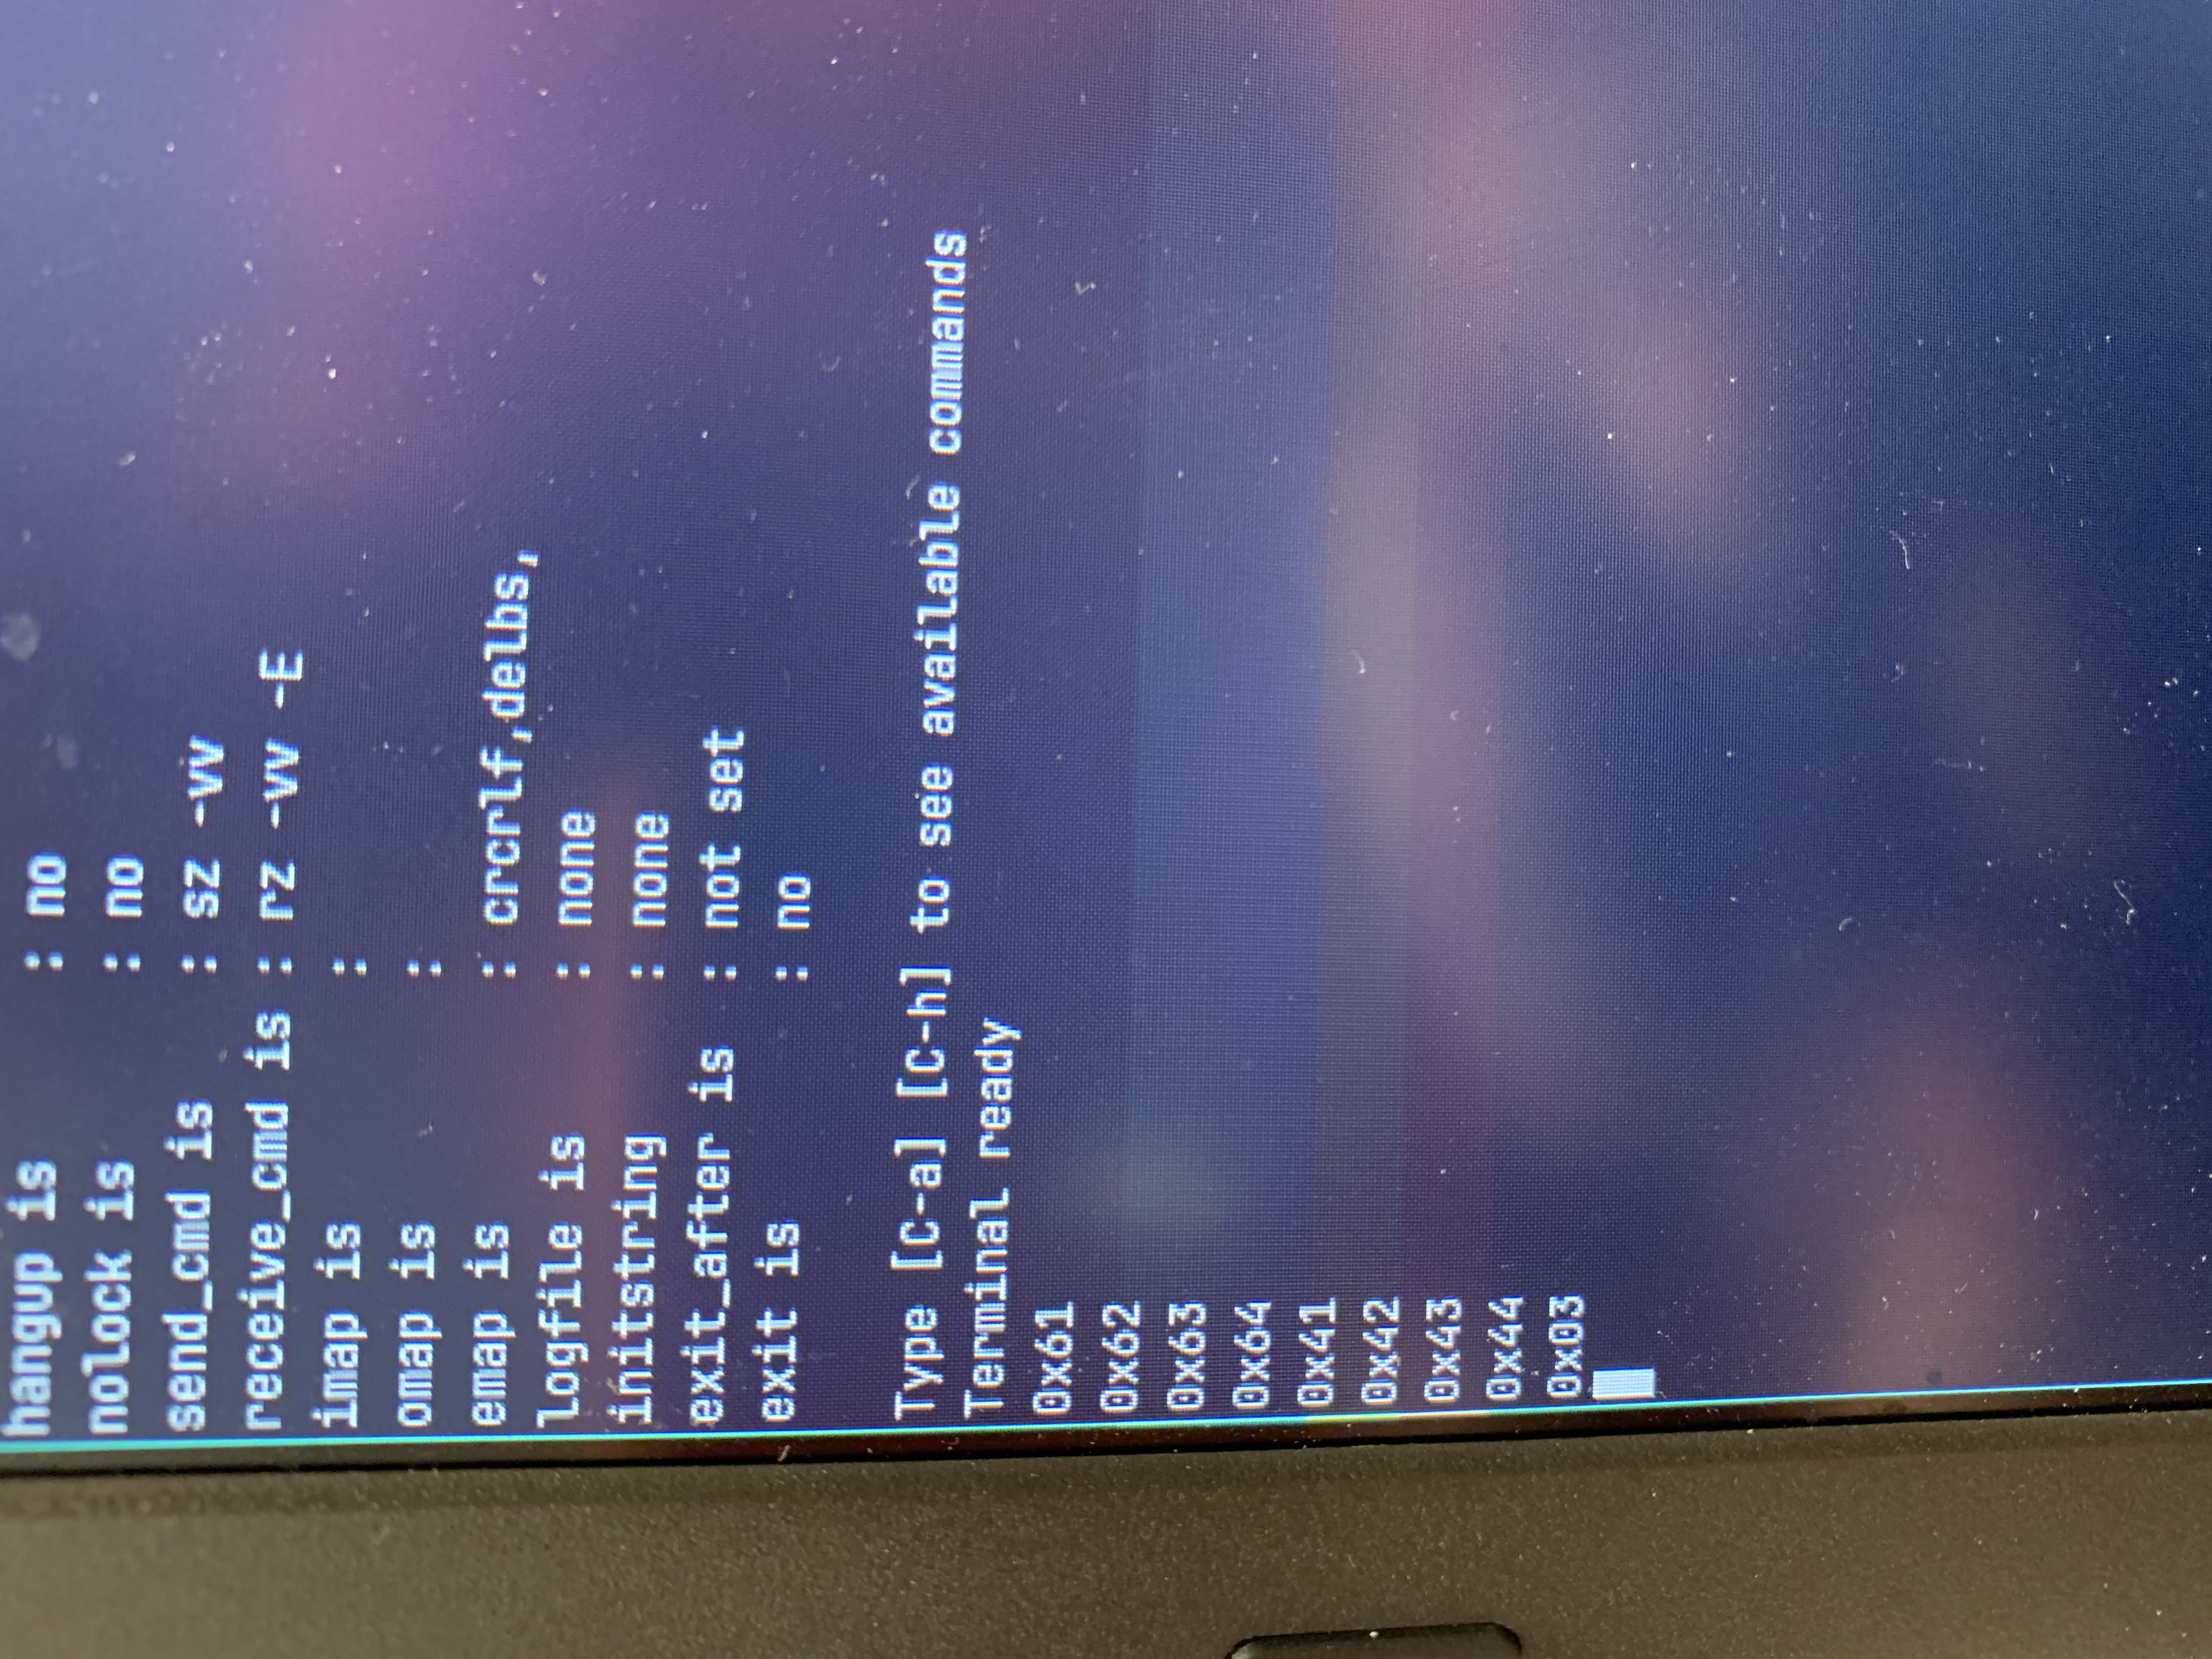
\includegraphics[scale=.1,angle=-90]{./images/1.jpg}
\end{document}
